\begin{activity} \label{A:11.8.6} 
\ba
	\item Find a set of spherical coordinates of the point whose Cartesian coordinates are $(-1, 1, 1)$. Draw a picture to illustrate all of the coordinates.
	
	
	
	\item Find the Cartesian coordinates of the point whose spherical coordinates are $(\rho, \theta, \phi) = \left(2, \frac{\pi}{6}, \frac{\pi}{3}\right)$. Draw a picture to illustrate all of the coordinates.
	
	
	
	\ea

\end{activity}
\begin{smallhint} 

\end{smallhint}
\begin{bighint}

\end{bighint}
\begin{activitySolution}
\ba
	\item We have $\rho = \sqrt{(-1)^2+1^2+1^2} = \sqrt{3}$, $\tan(\theta) = -1$, and $\cos(\phi) = \frac{1}{\sqrt{3}}$. Since $(-1,1)$ is in the second quadrant, we have $\theta = \frac{3\pi}{4}$, and the value of $\phi$ is $\arccos\left(\frac{1}{\sqrt{3}}\right) \approx 0.955$.  So $\left(\frac{1}{\sqrt{3}}, \frac{3\pi}{4}, \arccos\left(\frac{1}{\sqrt{3}}\right)\right)$ is a set of spherical coordinates of the point whose Cartesian coordinates are $(-1, 1, 1)$, as illustrated in the figure below. 
\begin{center}
\resizebox{!}{2.0in}{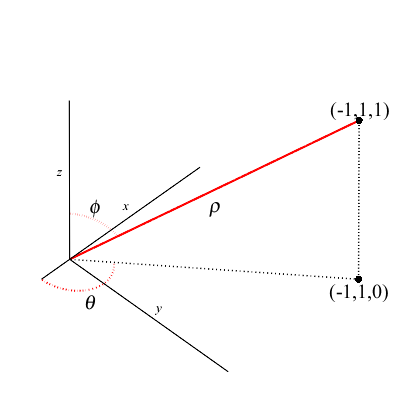
\includegraphics{11_8_spherical_1}}
\end{center}	
	
	
	\item Translating spherical coordinates to Cartesian coordinates we have 
\begin{align*}
x &= 2 \sin\left(\frac{\pi}{3}\right)\cos\left(\frac{\pi}{6}\right) = \frac{3}{2} \\
y &= 2 \sin\left(\frac{\pi}{3}\right)\sin\left(\frac{\pi}{6}\right) = \frac{\sqrt{3}}{2} \\
z &= 2 \cos\left(\frac{\pi}{3}\right) = 1.
\end{align*}
So the Cartesian coordinates of the point whose spherical coordinates are $\left(2, \frac{\pi}{6}, \frac{\pi}{3}\right)$ are $\left(\frac{3}{2}, \frac{\sqrt{3}}{2}, 1\right)$ as illustrated below. 
\begin{center}
\resizebox{!}{2.0in}{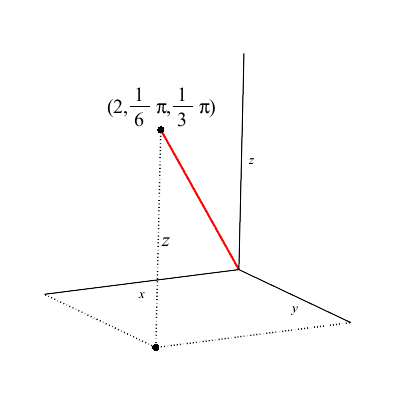
\includegraphics{11_8_spherical_2}}
\end{center}	
	
	
	
	\ea
\end{activitySolution}
\aftera
